\documentclass[10pt]{article}
\usepackage{a4wide}
\usepackage[final]{epsfig}

\parskip0.5\baselineskip
\sloppy

\def\scaledeps#1{\resizebox{\textwidth}{!}{\includegraphics{#1}}}
\def\centeredeps#1{\hbox to \textwidth{\hss\includegraphics{#1}\hss}}

% '_' is used very often in identifies but never as subscript... make
% it a normal character
\catcode`\_=12
\catcode`\&=12
\catcode`\^=4 % caret is alignment tab

% substitute non-bold slantex for non-existing cmtt/bx/sl (default is cmtt/m/n)
\DeclareFontShape{OT1}{cmtt}{bx}{sl}{<->ssub*cmtt/m/sl}{}

\def\slash{\texttt{\discretionary{/}{/}{}}}

\def\class#1{\texttt{#1}}
\def\type#1{\texttt{#1}}
\def\val#1{\texttt{#1}}
\def\var#1{\texttt{\slshape{#1}}}
\def\meth#1{\texttt{#1}()}
\def\func#1{\texttt{#1}()}
\def\tag#1{\textsc{#1}}
\def\prog#1{\texttt{#1}}
\def\file#1{\texttt{#1}}
\def\excp#1{\texttt{PkgDb#1Excp}}

\def\true{\val{true}}
\def\false{\val{false}}


\def\novsp{\vspace{-\baselineskip}}

\def\csection#1{\section{\class{#1}}\currentclass{#1}}
\def\cssection#1{\subsection{\class{#1}}\currentclass{#1}}
\def\currentclass#1{\global\def\currclass{\class{#1}}}
\def\headeris#1{Defined in: \texttt{<PkgDb/#1>}\par\noindent}

\def\ctypedef#1#2{%
  \subsubsection*{\mbox{Type: \texttt{typedef #1 \underline{#2}}}}%
  \novsp}
\def\ctype#1{%
  \subsubsection*{\mbox{Type: \texttt{\currclass::\underline{#1}}}}%
  \novsp}
\def\cmem#1#2{%
  \subsubsection*{\mbox{Member: \texttt{#1 \underline{#2}}}}%
  \novsp}
\def\cmeth#1#2#3{%
  \subsubsection*{\mbox{Method: \texttt{#1 \currclass::\underline{#2}(#3)}}}%
  \novsp}
\def\cfriend#1#2#3{%
  \subsubsection*{\mbox{Friend: \texttt{friend #1 \underline{#2}(#3)}}}%
  \novsp}
\def\cconst#1#2{%
  \subsubsection*{\mbox{Constructor: \texttt{%
    \currclass::\underline{\currclass}(#2)}}}%
  \novsp}

\def\synopsis#1{\par\vspace{\parskip}\noindent%
  \mbox{\textbf{Synopsis}: \texttt{#1}}\begin{description}}
\def\option#1#2{\item[Option: \texttt{-#1} \var{#2}]\ \\}
\def\arg#1{\item[\var{#1}]\ \\}
\def\endsynopsis{\end{description}}

\def\RPMLIBPATH{\file{rpm}}
\def\PKGDBBINPATH{\file{bin}}
\def\PKGDBBINPATH{\file{bin:tools}}
\def\PKGDBVLIBPATH{\file{PHI}}
\def\PKGDBULIBPATH{\file{PHI}}
\def\RPMDBFILENAME{\file{packages.rpm}}
\def\ICACHEFILENAME{\file{installed-cache}}
\def\REQFILESFILENAME{\file{required-files}}
\def\OVERRIDESFILENAME{\file{overrides}}
\def\ALTDEFAULTSFILENAME{\file{alternative-defaults}}
\def\INFOFILENAME{\file{PACKAGE-INFOS}}
\def\RELEASEFILENAME{\file{RELEASE}}
\def\RCACHEPREFIX{\file{cache_}}
\def\RRELEASEPREFIX{\file{release_}}
\def\ICACHEPROG{\file{pkg-installed-cache}}
\def\MKSUMPROG{\file{pkg-rpm2sum}}
\def\ASCIITOSUMPROG{\file{pkg-ascii2sum}}
\def\SUMTOASCIIPROG{\file{pkg-sum2ascii}}
\def\ICACHEPROG{\file{pkg-installed-cache}}
\def\MKSUMPROG{\file{pkg-rpm2sum}}
\def\ASCIITOSUMPROG{\file{pkg-ascii2sum}}
\def\SUMTOASCIIPROG{\file{pkg-sum2ascii}}

\parskip0.5\baselineskip
\sloppy

\begin{document}

\begin{center}
{\Large\bf
\texttt{libPkgDb} Documentation \\[\baselineskip]
}
{\large
Roman Hodek \texttt{<Roman.Hodek@informatik.uni-erlangen.de>} \\
December 1999
}
\end{center}
\vspace{1cm}

\tableofcontents
\newpage

% ===========================================================================

\section{Implementation Classes}

The classes described here are used in the implementation of the
exported classes. Nevertheless, libPkgDb users can use them if they
find them useful.

% ---------------------------------------------------------------------------

\subsection{\class{hash<key,val>} and \class{noval_hash<key>}}
\currentclass{hash}
\headeris{hash.h}

Hashes are one of the fundamental containers. Unfortunately, STL
doesn't define them. My implementation of hashes has the special
property that the number of buckets used is extended dynamically if
the average list length in a bucket becomes too long. This way, access
times to hash elements doesn't become too poor while not using too
much space for small hashes.

Sometimes also hashes are needed where the keys have meaningful no
associated data, but the presence of the key is enough information.
Those are modeled with an extra class \class{noval_hash}. Both,
\class{hash} and \class{noval_hash} are derived from
\class{basic_hash}, which implements most things. \class{noval_hash}
is separate because C++ doesn't allow to use declare e.g.
\texttt{hash<keytype,void>}.

\ctypedef{list_elem}{list_type}
Type of elements in a bucket list (contained type is template parameter).

\ctypedef{vector<list_elem*>}{vector_type}
Vector of buckets, each pointing to a list of elements with the same
hash value.

\ctypedef{hash_iterator<list_elem>}{iterator}
\ctypedef{hash_iterator<const list_elem>}{const_iterator}
Types of iterators for hashes.

\cconst{hash}{size_type size = 31, hashfun_t f = hashfun}
Constructs a typical empty hash. The initial number of buckets can be
selected with \var{size}, but this is usually not necessary as the
hashes are self-expanding. The second argument \var{f} can be a
special hash function of elements of the key type. In the formal case,
a properly overloaded instance of \func{hashfun} is used. I.e., you
should declare a \func{hashfun} for your key type before using a hash.

\cconst{hash}{const hash& S}
\cmeth{hash&}{operator=}{const hash& S}
Normal copying mechanisms.

\cmeth{iterator}{begin}{}
\cmeth{iterator}{end}{}
STL-compatible iterator returning methods.

\cmeth{void}{clear}{}
Makes the hash empty.

\cmeth{bool}{exists}{const Key& k}
Returns \true\ if a key equal to \var{k} exists in the hash.

\cmeth{list_type*}{insert}{const Key& k, const T& v}
\cmeth{list_type*}{insert}{const iterator& i}
\cmeth{list_type*}{insert}{const list_type *e}
Inserts a new element into the hash. Key and value are either given
directly or can be passed via an iterator or an \type{list_type*}.
If the key already existed, the old value is {\em not} overwritten. In
that case, the old (key,value) pair is returned.

\cmeth{T&}{operator[]}{const Key& k}
The subscript operator calls \meth{insert} for the given key and the
default object of the value type. It returns a reference to the value
for the key in the hash, no matter if the key already existed or had
to be created. This means you can use it for inserting values into the
hash like
\begin{quote}
\begin{verbatim}
hash<string,int> myhash;
myhash["abc"] = 1;
myhash["def"] = 2;
\end{verbatim}
\end{quote}
or you can use it to get values out of the hash:
\begin{quote}
\begin{verbatim}
if (myhash["xyz"] < 5) /* ... */
\end{verbatim}
\end{quote}
But beware that in case the key didn't exist, an default object of the
value type is returned and no error or exception. (The default object
is the one created by calling the constructor with no arguments.)

\cmeth{bool}{erase}{const Key& k}
Deletes the key \var{k} (and its value). It returns \false\ if
actually nothing has been deleted because the key didn't exist,
\true\ otherwise.

\cmeth{bool}{erase}{const iterator& i}
Like above deletes a (key,value) pair, but this time the key is passed
via an iterator.

\cmeth{size_type}{size}{}
Returns the number of elements in the hash.

\cmeth{size_type}{max_size}{}
Returns the number of buckets the hash currently uses. (This is a bit
different from the usual meaning\dots)

\cmeth{bool}{empty}{}
Returns \true\ if the hash has no elements stored.

\cmeth{void}{swap}{hash& s}
STL-like swap contents with another hash.

\cmeth{void}{statistics}{}
Print some statistics about the hash, including the elements/bucket
ratio.


% ---------------------------------------------------------------------------

\cssection{UniqStr}
\headeris{UniqStr.h}

\class{UniqStr} implements a store for strings, where is string is
stored only once. This means that for strings with the same contents,
the \meth{add} method always returns the same pointer. This allows
efficient comparison of strings for equality. Another application is
as a set of strings. When you add the same string multiple times, it
still will be in the store only once.

\class{UniqStr} uses an internal class \class{UniqStrInternal} as key
type for the hash. This class contains the \texttt{char *} itself and
a comparison operator that calls \func{strcmp}, so that equivalent
strings can be identified by the hash.

\ctypedef{noval_hash<UniqStrInternal>}{UniqStrHash_type}
Type of the string store.

\cmem{UniqStrHash_type}{UniqStrHash}
The string store itself. It is \texttt{protected} so that derived
classes can use it in additional ways.

\cmeth{const char *}{add}{const char *p = ""}
Add a string to the store and returns a unique pointer for the string.
I.e., if the string already existed, a pointer to the already stored
string is returned.


% ===========================================================================

\section{Basic Classes}
The classes below represent the data libPkgDb works with.

% ---------------------------------------------------------------------------

\cssection{PkgName}
\headeris{PkgName.h}

\class{PkgName} represents a package name. To save memory and to make
algorithms more efficient, the names are represented as unique
\type{char *}s with help by the \class{UniqStr} class. The comparison
operators only need to compare the pointers and thus are cheap.

\cmem{static UniqStr}{PkgNameHash}
The hash for mapping names to unique pointers (private; only one hash
needed for all names, thus static!)

\cconst{PkgName}{const char *n = ""}
Creates a new hash entry if \var{n} isn't already stored, otherwise
re-uses the old name.

\cmeth{bool}{operator==}{const PkgName& n2}
\cmeth{bool}{operator!=}{const PkgName& n2}
Cheap comparisons.

\cmeth{}{operator const char*}{}
Return name as \type{const char *}, so that it can be printed\dots

\cfriend{ostream&}{operator<<}{ostream&, const PkgName&}
For printing \class{PkgName}s



% ---------------------------------------------------------------------------

\cssection{PkgEdition}
\headeris{PkgEdition.h}

A \class{PkgEdition} represents version, release, and epoch of a
package. Since these three entities are used together for comparisons,
they're stored together. An edition is what you usually would call the
``version'', but this term in RPM parlance means the upstream version
only. To avoid misunderstandings, the new term ``edition'' has been
invented.

\class{PkgEdition} also supports two special values: \val{MAXIMUM} and
\val{UNSPEC}. A \val{MAXIMUM} edition is greater than any other. An
\val{UNSPEC} edition doesn't compare in any way with any other
edition, i.e. any comparison operator returns \false\ if an
\val{UNSPEC} takes part. (Exception: two \val{UNSPEC} editions are
equal.) These values are used to handle some specialties of providing
and obsoleting.

\cconst{PkgEdition}{const char *v = "", const char *r = NULL}
Constructs an edition without an epoch. The release \var{r} can be
empty. The version \var{v} can be left out, too, to allow construction
of default objects.

\cconst{PkgEdition}{int e, const char *v, const char *r = NULL}
Constructs an edition with epoch the same way as above.

\cconst{PkgEdition}{PkgEdition::type_enum t}
This is needed for constructing \val{MAXIMUM} and \val{UNSPEC}
versions, like:
\begin{quote}
\begin{verbatim}
PkgEdition( PkgEdition::MAXIMUM );
PkgEdition( PkgEdition::UNSPEC );
\end{verbatim}
\end{quote}

\cconst{PkgEdition}{const PkgEdition& e}
\cmeth{PkgEdition}{operator=}{const PkgEdition& e}
Normal copying mechanisms.

\cmeth{const char *}{version}{}
Returns the version part as C string. \val{UNSPEC} and \val{MAXIMUM}
editions return \verb|-*-UNSPEC-*-| and \verb|-*-MAXIMUM-*-|, resp.,
for printing them.

\cmeth{const char *}{release}{}
Returns the release part as C string. An non-existing release return
the empty string.

\cmeth{bool}{has_epoch}{}
Returns \true\ if the object has a release.

\cmeth{int}{epoch}{}
Returns the epoch part. If the edition doesn't contain an epoch, 0 is
given back.

\cmeth{bool}{has_epoch}{}
Returns \true\ if the object has an epoch.

\cmeth{bool}{is_unspecified}{}
Returns \true\ if the object is an \val{UNSPEC} edition.

\cmeth{bool}{is_maximum}{}
Returns \true\ if the object is a \val{MAXIMUM} edition.

\cmeth{bool}{compare}{rel_op op, const PkgEdition& e2}
General method for comparisons. \var{op} can be one of \val{EQ},
\val{NE}, \val{LT}, \val{LE}, \val{GT}, or \val{GE}. Usually
comparison operators are more convenient, but here you can pass the
relation operator as parameter.

\cmeth{bool}{operator==}{const PkgEdition& e2}
\cmeth{bool}{operator!=}{const PkgEdition& e2}
\cmeth{bool}{operator<}{const PkgEdition& e2}
\cmeth{bool}{operator<=}{const PkgEdition& e2}
\cmeth{bool}{operator>}{const PkgEdition& e2}
\cmeth{bool}{operator>=}{const PkgEdition& e2}
Comparison operators, call \meth{compare}.

\cmeth{string}{as_string}{}
Returns a \class{string} representation of the edition. Version and
release are concatenated with a dash (`\val{-}') as usual. If an epoch
is present, it is prefixed to the string, delimited by a colon
(`\val{:}'). An example representation is \val{1:2.0.24-2}.

\cmeth{}{operator string}{}
Same like \meth{as_string} as conversion operator.

\cfriend{ostream&}{operator<<}{ostream&, const PkgEdition&}
For directly printing editions.


% ---------------------------------------------------------------------------

\cssection{PkgNameEd}
\headeris{PkgName.h}

This class simply combines a \class{PkgName} and a \class{PkgEdition}.
It is used, e.g., as key type for hashes.


% ---------------------------------------------------------------------------

\cssection{PkgRelation}
\headeris{PkgRelation.h}

A \class{PkgRelation} represents a relation between packages, as used
in \tag{Requires}, \tag{Conflicts}, \tag{Provides}, and
\tag{Obsoletes}. There is always a package name as target of the
relation, and optionally an edition relation (comparison operator plus
compared edition). The non-presence of an edition relation is
represented by a comparison operator \val{NONE}.

The matching of two relations needs special mentioning: if you imagine
editions ordered on a ray that is infinite at both end, just like real
numbers, a relation is a subset on this ray (see
figure~\ref{editionray}). Two relations match if the intersection of
their subsets is not empty. In less mathematical terms this means this
means, e.g., that a \val{Requires: foo >= 1.2} matches a \val{Provides:
foo < 2.0}.

A relation with operator \val{NONE} has the whole set of editions
(let's call it $E$) associated. The unspecified version is a special
value outside the ordering of normal editions. This means that it
doesn't intersect with any subset, but it is included in the whole set
$E$. So a \val{Requires: foo} matches \val{Provides:
foo = -*-UNSPEC-*-}. The maximum version can be considered $+\infty$.
It is greater than every other edition and thus matches any $>$ or
$\ge$ relation, but no other one.

\begin{figure}
\centeredeps{relationmatch.eps}
\caption{Matching of Relations}
\label{editionray}
\end{figure}

\cconst{PkgRelation}{const PkgName& n, rel_op o, const PkgEdition& e}
Constructs a relation by simply putting together its components.

\cmeth{const PkgName&}{name}{}
\cmeth{PkgName&}{name}{}
Returns the target name of the relation.

\cmeth{rel_op}{op}{}
Returns the relation operator.

\cmeth{const PkgEdition&}{edition}{}
\cmeth{PkgEdition&}{edition}{}
Returns the edition taking part in the relation.

\cmeth{bool}{matches}{const PkgRelation& rel}
Returns \true\ when two relations match each other (see above).

\cmeth{bool}{matches}{const Package* pkg}
Basically the same as above, but it compares the object with the
self-providing relation of a package. The self-providing relation is
that each package provides its own name \val{=} its edition.

\cmeth{bool}{operator==}{const PkgRelation& r2}
\cmeth{bool}{operator!=}{const PkgRelation& r2}
Comparison of two relations. They're considered equal if their
components are equal. If the operator is \val{NONE}, then the editions
don't matter and aren't compared.

\cfriend{ostream&}{operator<<}{ostream&, const PkgRelation&}
For printing relations. The output format is like:
\begin{quote}\tt
foo \\
bar >= 1.2 \\
baz = 2.0 \\
gnat = -*-UNSPEC-*-
\end{quote}


% ---------------------------------------------------------------------------

\cssection{PkgRevRelation}
\headeris{PkgRevRel.h}

A \class{PkgRevRelation} describes a reverse relation, i.e. a package
relation with a back reference to the package owning the relation. It
is used as an auxiliary class by \class{PkgSet}.

Please note that the relation and the package are stored as pointers!
This is appropriate for \class{PkgSet} that only sets references to
the corresponding data in the package pool. But if you construct
temporary \class{PkgRevRelation} objects, beware that its components
do not end their lifetime before the \class{PkgRevRelation} object
does.

\cconst{PkgRevRelation}{const PkgRelation *r, const Package *p}
Construct a \class{PkgRevRelation} from its components. \var{r} can be
\val{NULL}. In this case, the \meth{relation} method returns the
self-providing relation of the package.

\cmeth{const PkgRelation}{relation}{}
Returns the relation component.

\cmeth{const Package *}{pkg}{}
Returns the package component.


% ---------------------------------------------------------------------------

\cssection{DistTag}
\headeris{DistTag.h}

\class{DistTag} objects are used to mark packages in the package pool
that belong together in some respect. A \class{DistTag} can be given
when adding a source to the package pool, and \class{PkgSet}s can be
built by referring to a list of \class{DistTag}s. The implementation
of a \class{DistTag} is simply a string.

\cconst{DistTag}{const char *p}
\cconst{DistTag}{const string &p}
\class{DistTag}s can be constructed from C string or \class{string}
objects.

\cconst{DistTag}{const DistTag& t2}
\cmeth{DistTag&}{operator=}{const DistTag& t2}
Normal copying mechanisms.

\cmeth{bool}{operator==}{const DistTag& t2}
\cmeth{bool}{operator=!}{const DistTag& t2}
To abstract from the underlying representation, the class provides
comparison operators.

\cmeth{}{operator const char*}{}
Converts a \class{DistTag} to a C string.

\file{DistTag.h} also defines the type \type{DistTagList} and
iterators for a (singly linked) list of \class{DistTag}s. There are
also two constant objects of this type, \val{NONE_Tag} and
\val{INSTALLED_Tag}. The latter is used as special value for the set
of currently installed packages.

There are also abbreviations for the generations of
\type{DistTagList}s: \func{DTagList\slshape{n}} takes \var{n} names
(of type \type{const char *}) and returns a \type{DistTagList}
consisting of tags for these names. \var{n} currently can be 1, 2, or
3. Similar functions \func{DTagListI\slshape{n}} additionally include
\val{INSTALLED_Tag} in the list. \var{n} can also be 0 here.


% ---------------------------------------------------------------------------

\cssection{Tag}
\headeris{DbHeader.h}

\class{Tag} is a C++ wrapper for an RPM tag value. It contains the tag
number, the type of the value(s), the number of values and a pointer
to the data. The \class{typedTag} template class provides easy access
to the values once the type of data is known.

\class{Tag} also handles the case where \func{headerGetEntry} calls
\func{malloc} to return the data (string arrays). It remembers if such
a \func{malloc} has been made and maintains a reference count to be
able to free the data later.

\cconst{Tag}{}
The default constructor constructs a \class{Tag} with all undefined fields.

\cconst{Tag}{const Tag& t2}
\cmeth{Tag&}{operator=}{const Tag& t2}
Normal copying mechanisms.

\cconst{Tag}{int_32 t, int_32 *val}
Construct a \class{Tag} with tag number \var{t} and one
\val{RPM_INT32_TYPE} value \var{*val}.

\cconst{Tag}{int_32 t, const char *val}
Construct a \class{Tag} with tag number \var{t} and one
\val{RPM_STRING_TYPE} value \var{val}.

\cconst{Tag}{int_32 t, const char **val}
Construct a \class{Tag} with tag number \var{t} and one
\val{RPM_STRING_ARRAY_TYPE} value \var{*val}.

\cconst{Tag}{int_32 t, int_32 type, const char **val, int_32 count}
\cconst{Tag}{int_32 t, int_32 type, void *val, int_32 count}
Construct a \class{Tag} with arbitrary contents.

\cmem{int_32}{tag}
\cmem{int_32}{type}
\cmem{int_32}{count}
\cmem{void *}{data}
These members are public and store the tag properties.

\cmem{int *}{refcnt}
This is the reference counter for tracking \func{malloc}ed data. If
the pointer is \val{NULL}, no counting is done. Otherwise,
\val{*refcnt} is the number of \class{Tag} objects referring to the
data array.

\cmeth{static string}{tagname}{int_32 tagno}
This static method translates tag numbers into tag names. If no
mapping for \var{tagno} is known, a string like ``\texttt{\#1032}'' is
returned, i.e. \var{tagno} itself is printed.

% ---------------------------------------------------------------------------

\cssection{typedTag}
\headeris{DbHeader.h}

The \class{typedTag} class provides easy access to the data in a
\class{Tag} structure. It is a template class that is specialized by
the type of data in the tag. The only member function is
\meth{operator[]}. Usage examples:
\begin{quote}
\begin{verbatim}
Tag tag_name = header[RPMTAG_NAME];
const char *name = typedTag<const char *>(tag_name)[0];

Tag tag_size = header[RPMTAG_SIZE];
int size = typedTag<int_32>(tag_size)[0];

Tag tag_files = header[RPMTAG_FILENAMES];
const char *thrd_file = typedTag<const char *>(tag_files)[2];
\end{verbatim}
\end{quote}
Valid indices for \meth{operator[]} are 0\dots\val{tag.count}. Many
tags contain only one value, so only index 0 can be used. The
representational difference between \val{RPM_STRING_TYPE} and
\val{RPM_STRING_ARRAY_TYPE} (\var{data} is either \type{const char *}
or \type{const char *[]}) is handled internally and not visible to the
user.

For convenience, there also exist \val{typedef}s for the most
often used template instantiations:
\begin{quote}
\begin{verbatim}
typedef typedTag<int_16> shTag;
typedef typedTag<int_32> iTag;
typedef typedTag<const char *> cpTag;
\end{verbatim}
\end{quote}
So the above example can be rewritten shorter as:
\begin{quote}
\begin{verbatim}
Tag tag_name = header[RPMTAG_NAME];
const char *name = cpTag(tag_name)[0];

Tag tag_size = header[RPMTAG_SIZE];
int size = iTag(tag_size)[0];

Tag tag_files = header[RPMTAG_FILENAMES];
const char *thrd_file = cpTag(tag_files)[2];
\end{verbatim}
\end{quote}


% ---------------------------------------------------------------------------

\cssection{DbHeader}
\label{pkgdb-dbheader}
\headeris{DbHeader.h}

The \class{DbHeader} class is the internal representation for package
data in caches. It happens to be identical to the ``header''
structures used by RPM 3.0, but this was only for ease of
implementation. There's no requirement that the external \prog{rpm}
program uses the same representation, nor does anything rely on the
concrete representation. It was just easy to copy some parts of RPM
code (\file{libPkgDb/pkgdbheader.cc} and
\file{libPkgDb/pkgdbheader.h}) and reuse it. Also conversion between
the two formats becomes easy :-) (For the concrete format of cache
files, see section~\ref{fileformat}.)

A \class{DbHeader} can be seen as a collection of \class{Tag}s. Member
functions are provided to retrieve tag values and to maintain the
contained tags. There is also an iterator \class{DbHeader::iterator}
to step through the tags sequentially.

\class{DbHeader} uses the type \type{PFD_t} for representing file
handles. On this type, the functions \func{pdfOpen}, \func{pdfClose},
\func{pfdLseek}, \func{pfdRead}, \func{pfdWrite}, \func{pfdValid}, and
\func{pfdFileno} are defined. They currently simply map to
\func{open}, \func{close}, \dots, but this can be changed later to
support compressed files via \val{libz} (e.g.).


\cconst{DbHeader}{const char *fn, PFD_t fd}
Constructs a \class{DbHeader} by reading the data (in binary
representation) from a file \var{fd} with name \var{fn}. The file name
and the offset in the file are stored inside the \class{DbHeader} and
can be used by the package pool later. This constructor is used to
sequentially read headers. It can throw \excp{} exceptions if the file
is at EOF or no valid header can be read at the current position.

\cconst{DbHeader}{const char *fn, off_t offset}
Constructs a \class{DbHeader} by reading the data (in binary
representation) from a file with name \var{fn} at offset \var{offset}.
This constructor can be used when you know in which file at which
offset the header is, as for example when \class{Package} reloads some
fields. This constructor can throw \excp{File} or \excp{} exceptions
if the file can't be opened or the seek or header read fails, resp.

\cconst{DbHeader}{PkgDb_Header hdr, const char *fn = "", off_t offs = -1}
Constructs a \class{DbHeader} from a raw \class{PkgDb_Header} (the
analogon to RPM's \class{Header} type). The file name and offset have
to be given explicitly.

\cconst{DbHeader}{}
Constructs an empty \class{DbHeader} with empty filename and offset -1.

\cconst{DbHeader}{const DbHeader& hdr}
\cmeth{DbHeader&}{operator=}{const DbHeader& hdr2}
Normal copying mechanisms.

\cmeth{const char *}{filename}{}
Returns the file name associated with the header.

\cmeth{off_t}{offset}{}
Returns the offset in the file \meth{filename}, where the header can
be found.

\cmeth{DbHeader::iterator}{begin}{}
Returns an iterator positioned at the first contained tag.

\cmeth{DbHeader::iterator}{end}{}
Returns an iterator positioned after the last contained tag.

\cmeth{const Tag}{get_tag}{int_32 tagno}
Retrieve the tag with number \var{tagno}. A \class{Tag} structure is
returned on success. If no tag with number \var{tagno} is contained in
the header, a \excp{NoTag} exception is thrown.

\cmeth{const Tag}{operator[]}{int_32 tagno}
Does the same as \meth{get_tag}, but is easier to use.

\cmeth{bool}{has_tag}{int_32 tagno}
Return \true\ is the header contains a tag with number \var{tagno}.

\cmeth{void}{add_tag}{const Tag& t}
Adds a new tag \var{t} to the header.

\cmeth{void}{extend_tag}{const Tag& t}
Adds the values in tag \var{t} to an existing tag with the same number
in the header. It is an error if the tag doesn't exist yet.

\cmeth{void}{modify_tag}{const Tag& t}
Removes the current values stored for \var{t.tag} and replaces them by
the new values in \var{t}.

\cmeth{void}{remove_tag}{int_32 tagno}
Removes a tag with number \var{tagno} from the header.

\cmeth{void}{write}{PFD_t fd}
Write the complete header (in binary format) to a file \var{fd}.

\cmeth{void}{read}{istream& is, int *lineno = NULL, bool is_override = false}
Reads a header in ASCII representation from the input stream \var{is}.
If \var{lineno} is not \val{NULL}, it is incremented for every newline
that is read, and the value is also used in error messages and
warnings.

If \var{is_override} is \true, the stream is parsed as an
override file. This means, on all non-key tags one of the override
markers \val{+}, \val{-}, or \val{!} is expected. Key tags are
\val{Name:}, \val{Version:}, \val{Release:}, \val{Epoch:}, and
\val{Edition:} which identify a package edition. The header will
contains two additional \type{int_32} array tags,
\val{PKGDBTAG_OVERRIDETAG} and \val{PKGDBTAG_OVERRIDEMODE}. The
formers contains a tag number (which exists in the header), and the
latter at the same index the override mode (add, remove, replace) that
should be applied to the tag.

\cfriend{istream&}{operator>>}{istream&, DbHeader&}
The shift-in operator is the same as the \meth{read} method with
\var{lineno} and \var{is_override} set to defaults.


% ===========================================================================

\csection{Package}
\headeris{Package.h}

\class{Package} is the representation of a package (in a specific
edition). Besides the basic data about the package (name, edition,
\dots) it contains all information necessary for dependency checking
(requires list, conflict list, \dots) and some auxiliary data (list of
distribution tags, summary, description, \dots).

Some of the contained data items (e.g., description, change log,
icons) need much space and/or are used only rarely. For this reason,
such items are loaded into memory at the time of the first reference,
not when the object is constructed. The load-on-demand items are:

\vspace{\baselineskip}
\begin{tabular}{|l|l|}\hline
access function ^ RPM tag name \\ \hline\hline
\texttt{packager()}			^ \texttt{RPMTAG_PACKAGER} \\
\texttt{distribution()}		^ \texttt{RPMTAG_DISTRIBUTION} \\
\texttt{vendor()}			^ \texttt{RPMTAG_VENDOR} \\
\texttt{sourcerpm()}		^ \texttt{RPMTAG_SOURCERPM} \\
\texttt{license()}			^ \texttt{RPMTAG_LICENSE} \\
\texttt{changelogname()}	^ \texttt{RPMTAG_CHANGELOGNAME} \\
\texttt{changelogtext()}	^ \texttt{RPMTAG_CHANGELOGTEXT} \\
\texttt{prein()}			^ \texttt{RPMTAG_PREIN} \\
\texttt{preun()}			^ \texttt{RPMTAG_PREUN} \\
\texttt{postin()}			^ \texttt{RPMTAG_POSTIN} \\
\texttt{postun()}			^ \texttt{RPMTAG_POSTUN} \\
\texttt{preinprog()}		^ \texttt{RPMTAG_PREINPROG} \\
\texttt{preunprog()}		^ \texttt{RPMTAG_PREUNPROG} \\
\texttt{postinprog()}		^ \texttt{RPMTAG_POSTINPROG} \\
\texttt{postunprog()}		^ \texttt{RPMTAG_POSTUNPROG} \\
\texttt{gif()}				^ \texttt{RPMTAG_GIF} \\
\texttt{xpm()}				^ \texttt{RPMTAG_XPM} \\
\texttt{icon()}				^ \texttt{RPMTAG_ICON} \\\hline
\end{tabular}
\vspace{\baselineskip}

For the load-on-demand feature, a \class{Package} stores the file name
of the cache it was loaded from, and the offset within this cache. If
a not yet loaded field is accessed, the header is read again and (at
least) the wanted field is loaded into memory. For efficiency, some
fields can be loaded together, i.e. if one is requested, some others
are made in-core fields, too. Currently all string type fields are
loaded if one is requested. The binary type fields (the last three)
load separately. The details of this can be easily changed if
there should be different requirements.

% ---------------------------------------------------------------------------

\subsection{Local Types}

\ctypedef{list<PkgRelation>}{PkgRelList_type}
Type returned by \meth{requires}, \meth{conflicts}, \meth{providers},
and \meth{obsoletes}. This is a sequence of \class{PkgRelation}s.

\ctypedef{PkgRelList_type::iterator}{PkgRelList_iterator}
\ctypedef{PkgRelList_type::const_iterator}{PkgRelList_const_iterator}
Iterators for \type{Package::PkgRelList_type}.

\ctypedef{vector<string>}{FileList_type}
\ctypedef{FileList_type::iterator}{FileList_iterator}
\ctypedef{FileList_type::const_iterator}{FileList_const_iterator}
Type returned by \meth{files} and iterators. It is a sequence of
\class{string}s.

\ctype{Provides_iterator}
\ctype{Provides_const_iterator}
This iterator steps through the provided names of a package. This
includes the package name itself (provided with relation
\val{= }\var{edition}), and all explicitly provided names (currently
always provided in unspecified edition). A \class{Provides_iterator}
is returned by \meth{all_provides_begin} and \meth{all_provides_end}.


% ---------------------------------------------------------------------------

\subsection{Constructors}

\cconst{Package}{const DbHeader&, bool read_all = false}
The constructor of a \class{Package} takes the data from a
\class{DbHeader}. If \var{read_all} is true, all fields are loaded,
even those that are usually load-on-demand. The \class{Package} also
stores the filename and offset contains in the \class{DbHeader} to be
able to reload fields later (the \class{DbHeader} objects doesn't need
to exist anymore at this point of time).

% ---------------------------------------------------------------------------

\subsection{Access to Information Fields}

All the methods below return the respective information field
contained in a \class{Package}.

\cmeth{const PkgName&}{name}{}
\allowbreak
\cmeth{const PkgEdition&}{edition}{}
\allowbreak
\cmeth{const FileList_type&}{files}{}
\allowbreak
\cmeth{const unsigned}{size}{}
\allowbreak
\cmeth{const string&}{summary}{}
\allowbreak
\cmeth{const string&}{group}{}
\allowbreak
\cmeth{const string&}{description}{}
\allowbreak
\cmeth{const string&}{packager}{}
\allowbreak
\cmeth{const string&}{distribution}{}
\allowbreak
\cmeth{const string&}{vendor}{}
\allowbreak
\cmeth{const string&}{sourcerpm}{}
\allowbreak
\cmeth{const string&}{sourcerpm}{}
\allowbreak
\cmeth{const string&}{license}{}
\allowbreak
\cmeth{const string&}{changelogname}{}
\allowbreak
\cmeth{const string&}{changelogtext}{}
\allowbreak
\cmeth{const string&}{prein}{}
\allowbreak
\cmeth{const string&}{preun}{}
\allowbreak
\cmeth{const string&}{postin}{}
\allowbreak
\cmeth{const string&}{postun}{}
\allowbreak
\cmeth{const string&}{preinprog}{}
\allowbreak
\cmeth{const string&}{preunprog}{}
\allowbreak
\cmeth{const string&}{postinprog}{}
\allowbreak
\cmeth{const string&}{postunprog}{}
\allowbreak
\cmeth{const string&}{gif}{}
\allowbreak
\cmeth{const string&}{xpm}{}
\allowbreak
\cmeth{const string&}{icon}{}
\allowbreak

\cmeth{const PkgRelList_type&}{requires}{}
\cmeth{const PkgRelList_type&}{conflicts}{}
\cmeth{const PkgRelList_type&}{provides}{}
\cmeth{const PkgRelList_type&}{obsoletes}{}
\allowbreak

\cmeth{const PkgRelList_iterator}{requires_begin}{}
\cmeth{const PkgRelList_const_iterator}{requires_begin}{}
\cmeth{const PkgRelList_iterator}{requires_end}{}
\cmeth{const PkgRelList_const_iterator}{requires_end}{}
(and similar functions for \val{conflicts}, \val{provides}, and
\val{obsoletes}).

% ---------------------------------------------------------------------------

\subsection{Containing Distributions}

\cmeth{const DistTagList&}{in_distribs}{}
Returns the list of distributions in which this package is contained.

\cmeth{void}{add_dist}{const DistTag& dist}
Tell the package that it is now also member of the distribution with
tag \var{dist}. (I.e., \var{dist} is added to the internal list of
distributions.)

\cmeth{bool}{is_in_distrib}{const DistTag& dist}
\cmeth{bool}{is_in_distrib}{const DistTagList& distlist}
Returns \true\ if the package is member of the distribution \var{dist}
or one of the distributions in the list \var{distlist}, resp.


% ---------------------------------------------------------------------------

\subsection{Adding New Provides}

\cmeth{const PkgRelation&}{add_provides}{PkgName name}
\cmeth{const PkgRelation&}{add_provides}{const char *name}
These two methods add a new \val{Provides: {\slshape name} = -*-UNSPEC-*-}
to the provides list of the package. They are used by the package pool
if new required files are known and old packages have to be rechecked
if they provide such a file.

% ---------------------------------------------------------------------------

\subsection{Requesting Provided Names}

\cmeth{Provides_iterator}{all_provides_begin}{}
\cmeth{Provides_iterator}{all_provides_end}{}
Begin and end iterators for a list of all names provided by this
package (see also description of \type{Provides_iterator}. For
example, if a package ``\val{foo}'', edition \val{1.0-1} provides
\val{bar} and \val{baz}, the iterator will return the following
relations:
\begin{quote}
\begin{verbatim}
foo = 1.0-1
bar = -*-UNSPEC-*-
baz = -*-UNSPEC-*-
\end{verbatim}
\end{quote}

\cmeth{PkgRelation}{self_provides}{}
Returns the {\em self-providing} relation of the package, i.e. the
relation that each package provides its own name in its current
edition. For example, the self-providing relation of a package
``\val{foo}'', edition \val{1.0-1} is ``\val{foo = 1.0-1}''.


% ---------------------------------------------------------------------------

\subsection{Misc}

\cfriend{ostream&}{operator<<}{ostream&, const Package&}
The shift-out operator prints a \class{Package} in a textual
representation (that can also be parsed by \meth{DbHeader::read}).

For each field, a field name is printed, followed by a colon and a
space. Then the value of the field follows, which may also be empty. A
field name must start at the beginning of a line. Whitespace (either a
space or a TAB character) at the start of a line denote a
continuation. For parsing, the whitespace is removed and the line is
concatenated with the previous one. For fields that have more than one
value, the single values are separated by commas or newlines. Printing
uses the separator which looks more usual for the field, parsing
doesn't care about it.

An example printout of a \class{Package} is:
\begin{quote}
\begin{verbatim}
Name: am-utils
Version: 6.0
Release: 4
Requires: /bin/sh, ld-linux.so.2, libc.so.6, libgdbm.so.1, libnsl.so.1
Size: 475216
Files:
 /etc/rc.d/init.d/amd
 /usr/bin/amq
 /usr/sbin/amd
 /usr/sbin/fsinfo
 /usr/sbin/mk-amd-map
 /usr/sbin/wire-test
Summary: Mounts network filesystems and local devices on demand.
Group: System/FileSystem
\end{verbatim}
\end{quote}

Please note that no data fields are loaded just for printing them. If
a field isn't in memory yet, it is left out.

\cmeth{const PkgDataSource&}{source}{}
This returns a \class{PkgDataSource} object that describes from where
the header of the package can be read (filename and offset). This is
the data needed for on-demand-loading of items.


% ===========================================================================

\csection{PkgDb}
\headeris{PkgDb.h}

The \class{PkgDb} class mainly is a store for a collection of package
descriptions (class \class{Package}). There is usually only one object
of this class, the global variable \val{PkgPool}\footnote{
  More than one \class{PkgDb} objects should work fine, but make no
  sense.},
which is already defined by \file{libPkgDb}.

Packages in the pool are identified by their name plus edition, i.e.
those two fields together are the keys into the database. It also
means that you can't store two different \class{Package} structures
that have the same name and edition (this doesn't make sense in
reality).

Every package in the pool has an attached list of distributions to
which it belongs. This can be used to build collections of packages
that belong together in the sense of \class{DistTag}s.

Besides storing package data, \class{PkgDb} also manages some global
information: overrides for package data, the default list of required
files, and alternative defaults.

% ---------------------------------------------------------------------------

\subsection{Local Types}
\ctypedef{PkgPool_type::iterator}{iterator}
\ctypedef{PkgPool_type::const_iterator}{const_iterator}
Iterators that step through all packages contained in the pool.

\ctypedef{list<const char *>}{ReqFiles_type}
\ctypedef{ReqFiles_type::iterator}{ReqFiles_iterator}
\ctypedef{ReqFiles_type::const_iterator}{ReqFiles_const_iterator}
This type (a list of strings) is used for enumerating the required
files lists (see below).

\ctypedef{list<PkgName>}{AltDefaultList}
\ctypedef{AltDefaultList::iterator}{AltDefaultList_iterator}
\ctypedef{AltDefaultList::const_iterator}{AltDefaultList_const_iterator}
This type is used for returning defaults for alternatives.

% ---------------------------------------------------------------------------

\subsection{Contained Packages}
\cmeth{add_source}{const char *path, DistTag tag = NONE_Tag}
This method adds a source path with packages to the pool. The packages
are all given the distribution tag \var{tag}. If \var{tag} is
\val{NONE_Tag}, it is tried to read the tag from the source path. For
details, see section~\ref{pkgdb-addsource} below.

\cmeth{add_installed_packages}{}
This calls \meth{add_source} with the special value
\val{INSTALLED_Tag} for \var{tag}. (\var{path} is an empty string, but
that is ignored.) It will read the packages currently installed on the
system into the pool.

\cmeth{const Package*}{get}{const PkgNameEd& ne}
\cmeth{const Package*}{get}{const PkgName& n, const PkgEdition& e}
\cmeth{const Package*}{operator[]}{const PkgNameEd& ne}
Retrieve a package description from the pool.

\cmeth{iterator}{begin}{}
\cmeth{iterator}{end}{}
Return iterators for stepping through all packages contained in the
pool.

% ---------------------------------------------------------------------------

\subsection{Additional Informations}
\cmeth{const ReqFiles_type&}{static_required_files}{}
Returns the static list of required files. (For details see
section~\ref{pkgdb-reqfiles}.)

\cmeth{const DbHeader*}{get_override}{PkgNameEd ne}
\cmeth{const DbHeader*}{get_override}{PkgName n, PkgEdition e}
Retrieve an override header for the package described by name and
edition. If no overrides are known for this packages, \val{NULL} is
returned.

\cmeth{AltDefaultList}{alternative_default}{PkgName name}
Retrieve the defaults for the virtual package name \var{name}. The
defaults are a list of package names that are preferred for the
virtual package in the returned order.

\cmeth{void}{clear_alternative_defaults}{}
Clears the list of alternative defaults.

\cmeth{void}{add_alternative_defaults}{const PkgName& name, const AltDefaultList& defaults}
Store a default list \var{defaults} for the virtual package
\var{name}. If a list for \var{name} already existed, it is
overwritten by the new list.

% ---------------------------------------------------------------------------

\subsection{Misc}

\cmeth{void}{attach_set}{PkgSet *set}
\cmeth{void}{detach_set}{PkgSet *set}
These methods are used by \class{PkgSet} objects to register and
deregister themselves at the package pool. A callback to
\class{PkgSet}s is needed whenever new required files become known.


% ---------------------------------------------------------------------------

\subsection{Adding Sources}
\label{pkgdb-addsource}

The package pool handles packages in terms of {\em package sources}.
Such a source is represented by a path name in the filesystem, but
that path not really needs to exist. In any case, the package data of
a source are always contained in a {\em cache}, usually named
``\INFOFILENAME''. The caches can either be pre-built, or they can be
generated dynamically.

If \meth{add_source} is called with \var{path} as argument,
\class{PkgDb} tries the following locations to find a cache for it:
\begin{enumerate}
\item
  It tries to open a file ``\var{path}\slash\INFOFILENAME''. If
  this file exists, it is used as the cache.

\item
  It tries to open a file 
  ``\PKGDBVLIBPATH\slash\RCACHEPREFIX\var{encoded-path}''. If that
  file exists, it is used as the cache.
\end{enumerate}
If all this fails, a new cache is built with the tool \MKSUMPROG. The
cache is written to ``\var{path}\slash\INFOFILENAME'', except
\var{path} doesn't exist or is not writable (e.g., if it's located on
a CD-ROM.) Then the cache is written to
``\PKGDBVLIBPATH\slash\RCACHEPREFIX\var{encoded-path}''.

If an existing cache has been found, it is checked that it's newer
than all \file{.rpm} files in \var{path}. If not, the cache is
rebuilt as described above. If \var{path} doesn't exist or contains no
\file{.rpm} files, the cache is considered up-to-date. This is
handy (for example) for caches that describe contents of a CD-ROM that
currently isn't mounted.

The \var{encoded-path} used above is an encoding of \var{path}, so
that it can be used as a file name. It is constructed by first
replacing all the characters
\begin{quote}
\verb^* ? [ ] < > | $ \ " ' & : ; _ =^
\end{quote}
with the MIME-like encoding ``\verb-=XX-'', where \verb-XX- is the
two-digit hexadecimal code for the character. In the next step, the
path separator `\slash' is replaced by an underscore `\texttt{_}'.

If the \var{tag} argument to \meth{add_source} is \val{NONE_Tag},
\meth{add_source} tries to find the proper tag for the source itself.
It looks for a file ``\var{path}\slash\RELEASEFILENAME'' or
alternatively
``\PKGDBVLIBPATH\slash\RRELEASEPREFIX\var{encoded-path}''. If
either exists, the first line of it is read (excluding the newline)
and used as the \class{DistTag} for the package in the source. If
there is no such file, \var{path} itself is used as the tag.

A special tag is \val{INSTALLED_Tag}. If it is used as \var{tag},
\var{path} is ignored and always the currently installed packages are
imported. There is a cache for those packages, too, it is
``\PKGDBVLIBPATH\slash\ICACHEFILENAME''. This cache is rebuilt
automatically if it is older than
``\RPMLIBPATH\slash\RPMDBFILENAME''. The tool used for rebuilding
it is \ICACHEPROG. Installed packages are usually added by
\meth{add_installed_packages}, which calls \meth{add_source} with the
appropriate parameters.

Here is a halfway realistic example for using caches and
\meth{add_source}: Assume the following files exist in \PKGDBVLIBPATH:
\nopagebreak
\begin{description}
\item[\RCACHEPREFIX\texttt{_cdrom_COL1.3}]\ \\
Cache for the \file{.rpm}s on a COL 1.3 CD-ROM
\item[\RRELEASEPREFIX\texttt{_cdrom_COL1.3}]\ \\
Contains ``\texttt{COL1.3}'' as distribution tag
\item[\RCACHEPREFIX\texttt{_cdrom_COL2.2}]\ \\
Cache for the \file{.rpm}s on a COL 2.2 CD-ROM
\item[\RRELEASEPREFIX\texttt{_cdrom_COL2.2}]\ \\
Contains ``\texttt{COL2.2}'' as distribution tag
\item[\RCACHEPREFIX\texttt{_cdrom_COL2.3}]\ \\
Cache for the \file{.rpm}s on a COL 2.3 CD-ROM
\item[\RRELEASEPREFIX\texttt{_cdrom_COL2.3}]\ \\
Contains ``\texttt{COL2.3}'' as distribution tag
\end{description}
The program using \file{libPkgDb} initializes the package pool with
the following calls:
\begin{quote}
\begin{verbatim}
add_source( "/cdrom/COL1.3" );
add_source( "/cdrom/COL2.2" );
add_source( "/cdrom/COL2.3" );
add_source( "/usr/local/lib/mypackages" );
add_installed_packages();
\end{verbatim}
\end{quote}
The first three statements will read the caches and release files from
\PKGDBVLIBPATH and thus will import three different distribution
versions. The fourth call is for local packages provided by the user.
If no cache exists yet in the path \file{/usr/local/lib/mypackages},
it will be generated automatically. It will also be rebuilt if a 
\file{.rpm} is changed or added in that directory. The last statements
imports the installed packages. Finally, the pool will contain
packages with five distribution tags: \val{COL1.3}, \val{COL2.2},
\val{COL2.3}, \val{/usr/local/lib/mypackages}, and \val{INSTALLED}.
The tag for the local packages might be different if the user has
provided a \RELEASEFILENAME\ file in \file{/usr/local/lib/mypackages}.

What source paths should be used when initializing the pool is in the
responsibility of the program using \file{libPkgDb}. It should either
have a configuration file for this, or offer the user some kind of
dialog, where he or she can configure what packages should be
available for installation.


% ---------------------------------------------------------------------------

\subsection{Required Files}
\label{pkgdb-reqfiles}

A special complication for dependency checking is the fact that RPM
packages can also require file names. Those are implicitly provided by
being member of the file list of the package. For RPM it is no trouble
to check those dependencies at install time, it just looks up the file
name in its internal database whether it's present. However, if you
want to check dependencies before actually installing (like
\file{libPkgDep} does) this isn't possible.

The correct way to handle required files would be to add a
\val{Provides:} relation for each file contained in a package. But
it's obvious that this would be overkill, as the vast majority of
files is never required. The provides lists would become that big that
performance would significantly suffer, not speaking of the memory
needed for storing all those unneeded provides. Therefore,
\file{libPkgDb} uses some more elaborated approach.

First, not every file can be required. File requirements are added by
\file{rpm} only for the interpreters of installation scripts. Thus,
all required files must be executable, or symlinks to executable
files. Next, there is usually a rather small set of about 10 or 15
files that are actually required. However, this set can change over
time, so we can't simply used a fixed list of names.

The approach of \file{libPkgDb} tries to combine efficiency in the
normal case with correctness for unusual cases. There are three
locations for lists of requires files:
\begin{enumerate}
\item
  The static list in \PKGDBULIBPATH\slash\REQFILESFILENAME. This
  list defines the ``normal'' required files and should cover at least
  all current cases. In other words, it's the basic set of required
  files.
\item
  Each cache contains a list of files required by packages in the
  cache.
\item
  The package pool maintains a list of files required by packages
  in the pool.
\end{enumerate}
The last two lists (in caches and in the pool) are initialized with
the static list. If a cache is read into the pool, \class{PkgDb}
compares their lists and takes appropriate action:
\begin{enumerate}
\item
  If the pool knows about a required file that the cache doesn't know
  about, every package described by the cache is checked if it
  contains that file. If yes, a \val{Provides: }\var{filename} is
  added to the package's relations.

  This covers the case that a new file has been added to the static
  list, and the cache still has been built with an older static list.
  The check also cares for consistency if some other cache has
  introduced new required files into the pool.

\item
  If the cache knows about a required file that the pool doesn't know
  yet, every package in the pool has to be rechecked if it contains
  that file. Like above, a provides relation is added if the file is
  found somewhere. The new required file is also added to the pools
  list.

  This covers the case that some package (in the cache) requires some
  new file, and this file hasn't been added to the static list yet.
\end{enumerate}

As you see, if the static list mentions all required files in all
caches, no additional checks for required files are necessary if
caches are merged into the pool. This is the efficient normal case.
This also means that the static list should be as up-to-date as
possible.

On the other hand, the scheme is still flexible enough if the static
list isn't properly updated, or if user-provided packages require yet
unregistered files. It involves a slight performance penalty, but this
(1) shouldn't happen often and (2) the operation isn't really that
expensive.

Another note: It is better not to delete files from the static list.
This would cause pool rechecks for those files if old caches (built
with the old static list) are imported.

For the checks, the package structures have to contain a file list.
Otherwise it wouldn't be possible to test if the package contains a
certain required file. As noted above, this file list can be
restricted to executable files or symlinks to them. This is managed by
the cache-building tools (\MKSUMPROG, \ICACHEPROG, and
\ASCIITOSUMPROG). They automatically trim down the file list to
regular executables (\verb'(mode & 0111) != 0 && S_ISREG(mode)') and
and symlinks (\verb'S_ISLINK(mode)'). If the regular target of a
symlink can be found in the same package and is not executable, that
symlink is omitted, too. This method reduces the file list stored in a
class \class{Package} to the required minimum. However, it also means
that you can't expected to see the real file lists of packages.

% ---------------------------------------------------------------------------

\subsection{Overrides}
\label{pkgdb-overrides}

\file{libPkgDb} provides {\em overrides} as possibility to overcome
metadata errors in old packages. If a package has been released and
distributed on CD, you can't change it's metadata (package relations
etc.) anymore, even if you later discover an error in those data. With
overrides, the wrong data can be corrected at least for the
applications using \file{libPkgDb}.

The override list looks like the ASCII representation of packages and
is stored in \PKGDBULIBPATH\slash\OVERRIDESFILENAME. The difference to
normal package data is that all non-key fields must have an override
mode prefix, which can be one of \texttt{+}, \texttt{-}, and
\texttt{!}. Key fields are \tag{Name}, \tag{Version}, \tag{Release},
\tag{Epoch}, and \tag{Edition}. They identify the package name and
edition where the changes should be applied. \tag{Edition} is just a
shorter alternative to write down the edition than using the three
tags \tag{Version}, \tag{Release}, and \tag{Epoch}. The key fields
must not have an override prefix.

Example for an override file entry:
\begin{quote}
\begin{verbatim}
Name: foo
Edition: 1.2-1
+Requires: foobar = 1.2
-Provides: fooold
!Conflicts: bar1, bar2
!Size: 1000
\end{verbatim}
\end{quote}

The \texttt{+} and \texttt{-} prefixes can be used only on array
fields (\tag{Requires}, \tag{Conflicts}, \tag{Provides},
\tag{Obsoletes}, and \tag{Filenames}). They add or remove the values
listed after the colon. For removing, an exact match of the name is
required, for \tag{Requires} and \tag{Conflicts} also of the relation
operator and edition. For example, if the original value is \val{foo =
1.2-1} and \val{foo >= 1.2-1} should be removed, the value isn't found
and nothing is deleted.

The \texttt{!} prefix means to completely replace a field with the
value from the override file. It can be applied to all fields.

Please note that also the cache-building tools read and use the
override list. So corrections are already included in caches built on
a system with an override file.

% ---------------------------------------------------------------------------

\subsection{Alternative Defaults}
\label{pkgdb-alternatives}

Sometimes there can be different packages for the same task, but at
most one of those packages can be installed at one time. Those
packages are called {\em alternatives}. When \file{libPkgDep}
encounters such an alternative, it will (under some circumstances) use
a default package.

For example, \file{cnews}, \file{inn}, and \file{leafnode} are all
news transport agents. The distribution might decide that \file{inn}
is the default NTA, or as second choice \file{cnews} if \file{inn}
can't be used for some reason.

Such decisions about defaults for alternatives should be stored in the
file \PKGDBULIBPATH\slash\ALTDEFAULTSFILENAME\ so that they are known
to \file{libPkgDep}. I considered the list of alternative defaults a
central service that should be managed by the package pool, therefore
is is part of \class{PkgDb} not \class{PkgDep}.

The alternatives list looks like:
\begin{quote}
\begin{verbatim}
news-transport-agent: inn cnews
mta: smail sendmail exim
c-compiler: gcc egcc pgcc
\end{verbatim}
\end{quote}
I.e., a virtual package name identifying the alternative is at the
start of the line, followed by a colon. All alternative packages must
provide that virtual name. Next come the names of packages that have
been chosen as defaults, in order of their preference and separated
by whitespace. Not all packages providing the virtual name have to be
listed. Those not mentioned will simply not be chosen if
\file{libPkgDep} works in a alternative mode that looks at defaults.


% ===========================================================================

\csection{PkgSet}
\headeris{PkgSet.h}

A \class{PkgSet} represents an unordered collection of packages. This
may be e.g. a set of currently installed packages, to be installed
packages, or ones that are available for installation. A package name
must be unique in a \class{PkgSet}, i.e. it is not possible to include
more than one version of a package\footnote{
  There were long discussions if this is a restriction for real life.
  The conclusion was that there are some rare cases where it might
  make sense to have more than one versions of a package installed
  (e.g. multiple kernel images), but those can easily be handled
  differently, too. And it makes life much easier to assume that only
  one version of a package can be installed or available etc.}.

Additionally to compounding packages, \class{PkgSet} has one more
important feature for dependency checking: It maintains reverse
indices of all package relations. I.e., you can ask the set what
packages (e.g.) require or provide a certain name. These reverse
indices are the core of an efficient dependency and consistency
checking.

% ---------------------------------------------------------------------------

\subsection{Local Types}

\ctypedef{hash<PkgName,const Package*>}{PkgList_type}
\ctypedef{PkgList_type::iterator}{iterator}
\ctypedef{PkgList_type::const_iterator}{const_iterator}
The internal type for the contents of the set and iterators for it.

\ctypedef{list<PkgRevRelation>}{RevRelList_type}
\ctypedef{RevRelList_type::iterator}{RevRelList_iterator}
\ctypedef{RevRelList_type::const_iterator}{RevRelList_const_iterator}
Type of the reverse index lists and iterators.

\ctypedef{hash<PkgName,RevRelList_type>}{InvRel_type}
\ctypedef{InvRel_type::iterator}{InvRel_iterator}
\ctypedef{InvRel_type::const_iterator}{InvRel_const_iterator}
Type of a reverse index (and iterators): It maps a package name to a
list of \class{PkgRevRelation}.

\subsection{Constructors}

\cconst{PkgSet}{}
Constructs an empty set.

\cconst{PkgSet}{const DistTagList& taglist}
Constructs a set that consists of all packages in the package pool
that have a distribution tag that is in \var{taglist}. This is a
convenient way to make a set of all packages that have certain tags.
If more than one edition of a package is selected this way, the newest
one is chosen and included in the set. (See also behavior of
\meth{add} below.)

\section{Maintenance}

\cmeth{void}{add}{const Package *pkg, bool force = false}
Adds a package to the set. If \var{force} is false, the package is
added only if no equal or newer edition is already member of the set.
This is handy most of the time, but can be overridden by passing
\true\ as second parameter. Then \var{pkg} is always added,
replacing a previous member of the set with the same name.

\cmeth{void}{remove}{const Package *pkg}
\cmeth{void}{remove}{PkgName name}
Removes a package from the set, identified either by a name or by a
package structure.

\cmeth{void}{new_provides}{const Package *pkg, const PkgRelation& prov}
This is called by \class{PkgDb} if new required files are provided.
The method updates the reverse index for the provides relation accordingly.

\subsection{Lookup}

\cmeth{bool}{includes}{const PkgName& name}
Returns \true\ if a package with name \var{name} is member of the set.

\cmeth{const Package *}{lookup}{PkgName name}
\cmeth{const Package *}{operator[]}{PkgName name}
These methods return that package structure for a member of the set,
identified by name. If \var{name} isn't included in the set,
\val{NULL} is returned.

\cmeth{iterator}{begin}{}
\cmeth{iterator}{end}{}
\cmeth{const_iterator}{begin}{}
\cmeth{const_iterator}{end}{}
Return iterators that step through all packages in the set.

\subsection{Reverse Indices}

\cmeth{const InvRel_type&}{required}{}
\cmeth{const InvRel_type&}{conflicted}{}
\cmeth{const InvRel_type&}{provided}{}
\cmeth{const InvRel_type&}{obsoleted}{}
These methods return the reverse indices for packages relations. The
returned value is a hash that can be indexed by a \class{PkgName}. For
example, to learn the names of all packages that require \val{foo}:
\begin{quote}
\begin{verbatim}
PkgSet pset;
// ...
const PkgSet::RevRelList_type& requires_foo = pset.required()[PkgName("foo")];
for( PkgSet::RevRelList_const_iterator p = requires_foo.begin();
     p != requires_foo.end(); ++p ) {
  cout << *p->pkg()->name << endl;
}
\end{verbatim}
\end{quote}

\cmeth{InvRel_iterator}{required_begin}{}
\cmeth{InvRel_const_iterator}{required_begin}{}
\cmeth{InvRel_iterator}{required_end}{}
\cmeth{InvRel_const_iterator}{required_end}{}
These return iterators for the reverse indices. With those, you can
step through all the keys of such an index.



% ===========================================================================

\section{File Format of Cache Files}
\label{fileformat}

The cache files created by \MKSUMPROG, \ASCIITOSUMPROG, and
\ICACHEPROG\ all share the same file format. They consist of at least
one {\em header} structures. The first header is for use by
\file{libPkgDb} and applies to the whole cache. All following headers
describe a single package (see figure~\ref{fig-header}).

\begin{figure}[htb]
\hbox to \textwidth{\hss\includegraphics[width=14cm]{header.eps}\hss}
\caption{Caches and Headers}
\label{fig-header}
\end{figure}

The header structures have the same format as those used by RPM 3.0.
But to stress the fact that it is still an internal format and doesn't
create any relation to any RPM version, the header format is described
here separately.

A header is basically a collection of {\em tags}. A tag is an
association of a {\em tag number} (giving data's meaning), a type (how
the data should be interpreted), the number of data items, and the raw
data, which is an arbitrary sequence of bytes. All multi-byte data in
a header are stored in network byte order (big endian).

A header has its own header with the following fields:
\begin{quote}
\begin{tabular}{|l|l|l|}
\hline
field			^ type			^ description \\
\hline
\val{magic}		^ \val{char[4]}	^ magic to identify an header (0x8e 0xad 0xe8 0x01) \\
\val{filler}	^ \val{int_32}	^ unused \\
\val{entries}	^ \val{int_32}	^ number of tag entries \\
\val{size}		^ \val{int_32}	^ size in bytes of the data section \\
\hline
\end{tabular}
\end{quote}
Directly after the header header follow \var{entries} tag structures
that look like
\begin{quote}
\begin{tabular}{|l|l|l|}
\hline
field			^ type			^ description \\
\hline
\val{tag}		^ \val{int_32}	^ tag number \\
\val{type}		^ \val{int_32}	^ type (see table below) \\
\val{count}		^ \val{int_32}	^ number of data items \\
\val{offset}	^ \val{int_32}	^ offset to data bytes, relative to data section \\
\hline
\end{tabular}
\end{quote}
After the tag structures, the data section immediately follows.
Possible types for tags are:
\begin{quote}
\begin{tabular}{|l|l|l|}
\hline
type name						^ number ^ description \\
\hline
\val{RPM_INT16_TYPE}			^ 3      ^ short integer (16 bit) \\
\val{RPM_INT32_TYPE}			^ 4      ^ integer (32 bit) \\
\val{RPM_STRING_TYPE}			^ 6      ^ null-terminated string \\
\val{RPM_BIN_TYPE}				^ 7      ^ unstructured binary data \\
\val{RPM_STRING_ARRAY_TYPE}		^ 8      ^ \var{count} null-terminated strings \\
\hline
\end{tabular}
\end{quote}

Other types defined by RPM are not used in the \file{libPkgDb} format.
A bit peculiar is the difference between \val{RPM_STRING_TYPE} and
\val{RPM_STRING_ARRAY_TYPE}: The former requires that \var{count} in the tag
structure is 1, but their representation in the data section is the
same: There are \var{count} concatenated null-terminated character
sequences. The real differences between the two types is the format
they're returned as: a single string as \type{char *}, an array as
\type{char **}, where the pointer array is \func{malloc}-ed.

The first header in a cache for \file{libPkgDb} currently contains two
tags: \val{PKGDBTAG_VERSION} (200000) and
\val{PKGDBTAG_REQUIRED_FILES} (200001). The former gives a version
identification that can be used later to enable compatibility modes or
the like. The latter is a string array storing all the required files
known to the cache. (See required files handling in
section~\ref{pkgdb-reqfiles}.)


% ===========================================================================

\section{Exceptions}
\headeris{Exception.h}

All exceptions that can be thrown by \file{libPkgDb} are of type
\excp{} or a derived class. A \excp{} object
simply stores an error description that can be printed. There is a
virtual \meth{print} method an a \val{<<} operator defined.

If you want to catch any exception, be sure to catch the exception
object by reference, so the virtual method correctly can be called.
For example:
\begin{quote}
\begin{verbatim}
try {
    // PkgDb calls...
}
catch( PkgDbExcp& excp ) {
    cerr << "Caught PkgDb exception: " << excp << endl;
    exit( 1 );
}
\end{verbatim}
\end{quote}

There are a few specialized subclasses of \excp{} that either store
additional data or indicate special kinds of errors:

\cssection{PkgDbFileExcp}

This type additionally stores an \val{errno} (as returned by the
underlying operating system functions) and is used for OS-related
errors. The print method calls \func{strerror} to translate the
\val{errno} into a string.

\cssection{PkgDbNoTagExcp}

Several methods that look up tags can throw this object to indicate
that the requested tag number does not exist. The object stores the
failed tag number and \meth{print} prints the tag name, or if the
number isn't known, the raw number.

\cssection{PkgDbReadTagExcp}

This is thrown only by \meth{DbHeader::read}. It indicates some kind
of parse error in the input stream. An additional data item indicates
the line number where the error happened.


% ===========================================================================

\section{Tools}

With \file{libPkgDb} come some tools that can read or write the cache
format defined by the library:

% ---------------------------------------------------------------------------

\subsection{\MKSUMPROG}

\MKSUMPROG\ builds a cache from the data in \file{.rpm} files.

\synopsis{\MKSUMPROG\ [-v] [-o \var{outfile}] \var{files-or-directories...}}
\option{v}{}
Verbose operation: print names of files processed. If given twice,
also enable informations about the required files handling.

\option{o}{outfile}
Write the resulting output cache to \var{outfile}, instead to the
default name \INFOFILENAME in the current directory.

\arg{files-or-directories}
You can give either the names of \file{.rpm} files to process to
\MKSUMPROG, or directories that are recursively searched for
\file{.rpm} files.

\endsynopsis

% ---------------------------------------------------------------------------

\subsection{\ICACHEPROG}

\ICACHEPROG\ build a cache for the currently installed packages. It
reads \RPMLIBPATH\slash\RPMDBFILENAME\ to do this.

\synopsis{\ICACHEPROG\ [-v] [-o \var{outfile-or-dir}]}

\option{v}
Verbose operation: print names of files processed. If given twice,
also enable informations about the required files handling.

\option{o}{outfile-or-dir}
Write the resulting output cache to \var{outfile-or-dir}, instead to the
default name \ICACHEFILENAME\ in the current directory. If
\var{outfile-or-dir} is a directory, \ICACHEFILENAME\ is created in
that directory.

\endsynopsis

% ---------------------------------------------------------------------------

\subsection{\SUMTOASCIIPROG}

\SUMTOASCIIPROG\ dumps the contents of a cache in human-readable ASCII
format. Each tag is printed in the format
\begin{quote}
\texttt{tagname: value}
\end{quote}
The \texttt{value} may span more than one line, the continuation lines
begin with a whitespace character. An empty line marks the border
between different packages.

\synopsis{\SUMTOASCIIPROG\ [-v] [-h] \var{cache-files...}}

\option{v}{}
Verbose mode: Also show the tags that are not always included in a
class \class{Package}, but are loaded on demand.

\option{h}{}
Also show the contents of the \file{libPkgDb} private header. It
currently contains a version number and the list of required files.
The private header is printed like a package before the real packages
in the cache.

\arg{cache-files}
An arbitrary number of cache files to dump.

\endsynopsis

% ---------------------------------------------------------------------------

\subsection{\ASCIITOSUMPROG}

\ASCIITOSUMPROG\ can convert the ASCII representation to a cache file.
The input format is (nearly\footnote{
  The difference is just that \ASCIITOSUMPROG\ accepts the
  \val{Edition:} pseudo tag that is never printed by \SUMTOASCIIPROG.})
the same like printed by \SUMTOASCIIPROG.
It has been described in detail in section~\ref{pkgdb-dbheader}.

\synopsis{\MKSUMPROG\ [-v] [-o \var{outfile}] [\var{ascii-files...}]}

\option{v}{}
Verbose operation: print names of files processed. If given twice,
also enable informations about the required files handling.

\option{o}{outfile}
Write the resulting output cache to \var{outfile}, instead to the
default name \INFOFILENAME in the current directory.

\arg{ascii-files}
An arbitrary number of ASCII representation files to convert. The
contents are all written to the same cache. If no \var{ascii-file} is
given, standard input is read.

\endsynopsis


% ===========================================================================

\section{Files}

\subsection{\INFOFILENAME}

This is the normal name of a cache file when adding a source path to
the package pool (see section~\ref{pkgdb-addsource}). It has to be in
standard cache format (see section~\ref{fileformat}) and is usually
generated by \MKSUMPROG. 

\subsection{\RELEASEFILENAME}

A \RELEASEFILENAME\ file can accompany a \INFOFILENAME\ and tells the
default release tag (\class{DistTag}) for packages in the cache. If
it's missing and the caller of \meth{add_source} hasn't supplied a
tag, the path name is used instead.

It simply contains a line of text that is used as the tag. All lines
except the first are ignored.

\subsection{\PKGDBVLIBPATH\slash\RCACHEPREFIX\texttt{*}}

\file{libPkgDb} uses files with this name pattern for storing
relocated caches. Caches have to relocated if the source path of the
\file{.rpm} files isn't writable, e.g. because it's on a CD-ROM. The
relocated cache file is tried if no \INFOFILENAME\ file exists in the
source path. The suffix of the name is generated following the rules
described in section~\ref{pkgdb-addsource}-

\subsection{\PKGDBVLIBPATH\slash\RRELEASEPREFIX\texttt{*}}

These are companions to \RCACHEPREFIX\texttt{*}. They tell the release
tag associated with the cache. However, those files are never
automatically generated and are useful only if caches are provided,
e.g., for older releases in \PKGDBVLIBPATH.

\subsection{\PKGDBVLIBPATH\slash\ICACHEFILENAME}

This file is again in standard cache format (see
section~\ref{fileformat}). It is the cached version of \RPMDBFILENAME.
The cache is rebuilt automatically by \file{libPkgDb} each time it is
found to be older than \RPMDBFILENAME.

\subsection{\PKGDBULIBPATH\slash\REQFILESFILENAME}

This is the default list of required files (see
section~\ref{pkgdb-reqfiles}). It contains a list of file names, one
per line. Example:
\begin{quote}
\begin{verbatim}
/bin/bash
/bin/csh
/bin/sh
/bin/tcsh
/bin/zsh
/sbin/ldconfig
/usr/bin/awk
/usr/bin/env
/usr/bin/expect
/usr/bin/expectk
/usr/bin/perl
/usr/bin/perl
/usr/bin/python
/usr/bin/wish
/usr/X11R6/bin/mkfontdir
\end{verbatim}
\end{quote}

\subsection{\PKGDBULIBPATH\slash\OVERRIDESFILENAME}

This file can contain overrides as described in
section~\ref{pkgdb-overrides}, where also the file format is
described. Basically, it looks like an ASCII representation of a
cache, but with override markers (\texttt{+}, \texttt{-}, and
\texttt{!}) before the non-key fields.

Example:
\begin{quote}
\begin{verbatim}
Name: adduser
Edition: 1.2-1
+Requires: foobar = 1.2

Name: qt
Edition: 1.42-2
-Requires: ld-linux.so.2

Name: adjtimex
Edition: 1.3-1
!Requires: ld-linux.so.3, libc.so.7
!Size: 1000
\end{verbatim}
\end{quote}

\subsection{\PKGDBULIBPATH\slash\ALTDEFAULTSFILENAME}

This file defines the defaults to be used if there are more than one
alternative for a virtual package name (see
section~\ref{pkgdb-alternatives}). It could look like:
\begin{quote}
\begin{verbatim}
mta: smail sendmail exim
c-compiler: gcc egcc pgcc
\end{verbatim}
\end{quote}

\end{document}


